\section{Proposed Cloud-based Buffer Bursts}
\label{sec:architecture}

%\begin
An overview of I/O burst buffer architecture is described in this section.
As we mentioned in the previous section, our model takes advantage of high throughput inside a system, and use buffer queue system in order to increase throughput between two systems.
%Two kinds of buffer are used in our I/O burst buffer architecture, the first one is in client computing node, first buffer user I/O in the same node, another one is in I/O buffer nodes.
The main idea is that some of computing nodes serve as a I/O buffer nodes in each system, for write I/O data, if buffer queue in I/O buffer nodes is not full, data can first be buffered in buffer queue in the same system, and then client can finish write operation without waiting data be finally transferred to storage system.
Actually, since many jobs use multiple nodes work together and the output of some nodes can be the
input of the others, so for most cases, output data will still be buffered in buffer queue until the whole job finished.
As for reading, if that file is stored in the buffer queue, compute nodes can read from I/O nodes through interconnection network.
In other cases (buffer queue is full when issue a write request or requested file is not stored in buffer queue when issue a read request we call it cache miss), a read from or write back operation described below will be executed. 

\subsection{Target Environment}
First, we introduce our target environment.
we target at common cloud environment like Amazon EC2, which compute node and data center are distributed geographically distributed.

\begin{itemize}
	\item All compute nodes are connected by large bandwidth and interconnection network, note network topology maybe different in each system, so topology is not specified here, interconnection network performance is measured by throughput.
	\item There is a shared storage for data sharing inside system, all compute nodes are connected
	with shared storage via Internet or other lower network, also the file system of shared storage is not specified and performance is measured by throughput.
\end{itemize}

\subsection{I/O Burst Buffer Architecture}

\begin{figure}[tb]
	\centering
	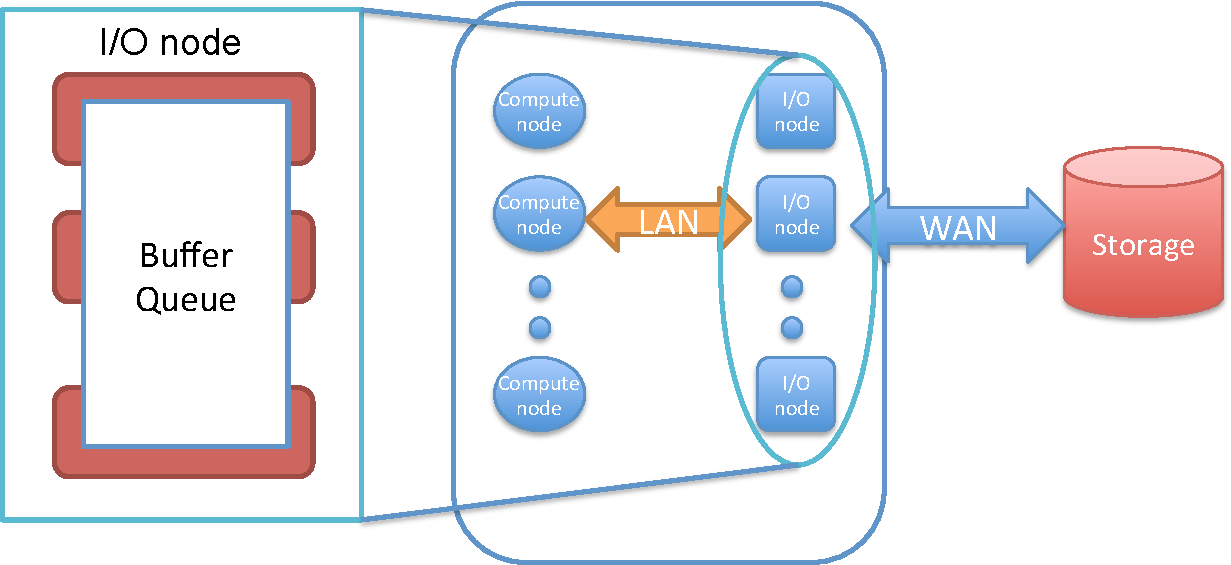
\includegraphics[width=8cm]{img/architecture_overview}
	\caption{overall illustrate of I/O Burst Buffer Architecture}
	\label{architecture:overview}
\end{figure}

There are two kinds of nodes in our I/O burst buffer architecture: \emph{compute nodes} and \emph{I/O burst nodes}, compute nodes run user's application and I/O burst nodes.
Public clouds usually provide several type of instance for difference purpose, some are compute
optimized (like C3 instances provided by Amazon) provides a high compute performance, some are memory optimized (such as R3 instances in Amazon EC2) provide a huge amount of memory (up
to 244GB in R3 family), also memory size can be easily expanded by using solid storage driver (SSD)
as a swap device, usually such instances have SSD inside.

Fig.~\ref{architecture:overview} shows an overall illustrate of I/O burst buffer architecture.